\section{Lezione 23}%
\label{sub:Lezione 23}
\subsection{Caos nei sistemi dissipativi}%
\label{sub:Caos nei sistemi dissipativi}
Sono stati proposti diversi scenari per studiare il caos nei sistemi dissipativi.
\subsubsection{Scenario di Landau-Hopf}%
\label{subsub:Scenario di Landau-Hopf}
Questo è stato proposto da Landau ed utilizza la \textbf{biforcazione di Hopf} che viene descritto sotto.\\
Si parte dal caso già studiato Hamiltoniano. Nei sistemi dissipativi al variare di un qualche parametro si ha l'"accensione" di nuove varietà che vanno a formare tori nello spazio delle fasi.\\ 
Questi tori crescono e nuovi tori nascono, in conclusione l'interazione di questi tori genera il caos. \\
Questa visione non ha una corrispondenza nelle situazioni sperimentali: non è questo quello che si osserva.
\paragraph{Biforcazione di Hopf}%
\label{par:Biforcazione di Hopf}
Nei sistemi dissipativi abbiamo spesso a che fare con mappe aventi autovalori complessi coniugati (vedi ad esempio pendolo smorzato). Nell'idea di Hopf le traiettorie non spiraleggiano verso un punto (il punto fisso) ma tendono a cadere su una varietà, come se il moto avvenisse all'interno di un potenziale dalla forma a sombrero. 
\begin{figure}[H]
    \centering
    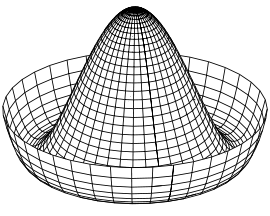
\includegraphics[width=0.3\textwidth]{figures/sombrero.png}
    \caption{\scriptsize Forma di un potenziale a sombrero (wikipedia).}
    \label{fig:figures-sombrero-png}
\end{figure}
\noindent
Vediamo che in una situazione del genere si forma un ciclo limite stabile sul fondo della buca.\\
Tuttavia, se prendiamo come esempio l'attrattore di Lorenz, l'oggetto non presenta dei tori: quando passa nei pressi di un punto critico l'oggetto non viene catturato su una varietà ma scappa via.\\
Proprio per questo si cerca spesso un meccanismo più credibile (rispetto a Landau-Hopf): 
\subsubsection{Meccanismo di Ruelle-Taken}%
\label{subsub:Meccanismo di Ruelle-Taken}
Il meccanismo è analogo a quello di Landau-Hopf ma le varietà finali su cui il moto può andare non sono dei tori ma sono dei frattali!\\
Quindi mentre prima si ipotizzava che il sistema evolvesse all'ordine (tori) adesso si ipotizza che il sistema evolva nel caos per il teorema accennato al fine della scorsa lezione (caos-frattale). Approfondiamo qui la struttura del teorema.
\begin{thm}[Axiom A]
    Prendiamo un diffeomorfismo $f: \ M\to M$. Il sistema che soddisfa i seguenti due punti:
    \begin{itemize}
	\item Ha un insieme $U:$ $\forall x \in U$ $|$ $\mu (f^h(U) \cap U) > 0 $ con $U$ iperbolico e compatto.\\
	    In altre parole per ogni punto in un insieme iperbolico e compatto (come la sfera unitaria senza buchi) ogni iterazione della mappa finisce nell'insieme stesso.
	\item L'insieme dei punti periodici di $f$ è denso in $U$ (dato un punto periodico di $f$ $\implies$ in un suo intorno ci sono punti periodici di $U$).
    \end{itemize}
    se giace su una varietà frattale allora è caotico (inteso come esponente di Lyapunov più grande maggiore di zero).\\
\end{thm}
\noindent
La dimostrazione si basa sul meccanismo di Stretching e Folding illustrato nella sezione \ref{sub:Mappa di Henon come meccanismo di Folding e Stretching}. \\
Un altra mappa interessante che illustra questo meccanismo è la Horseshoe:
\begin{figure}[H]
    \centering
    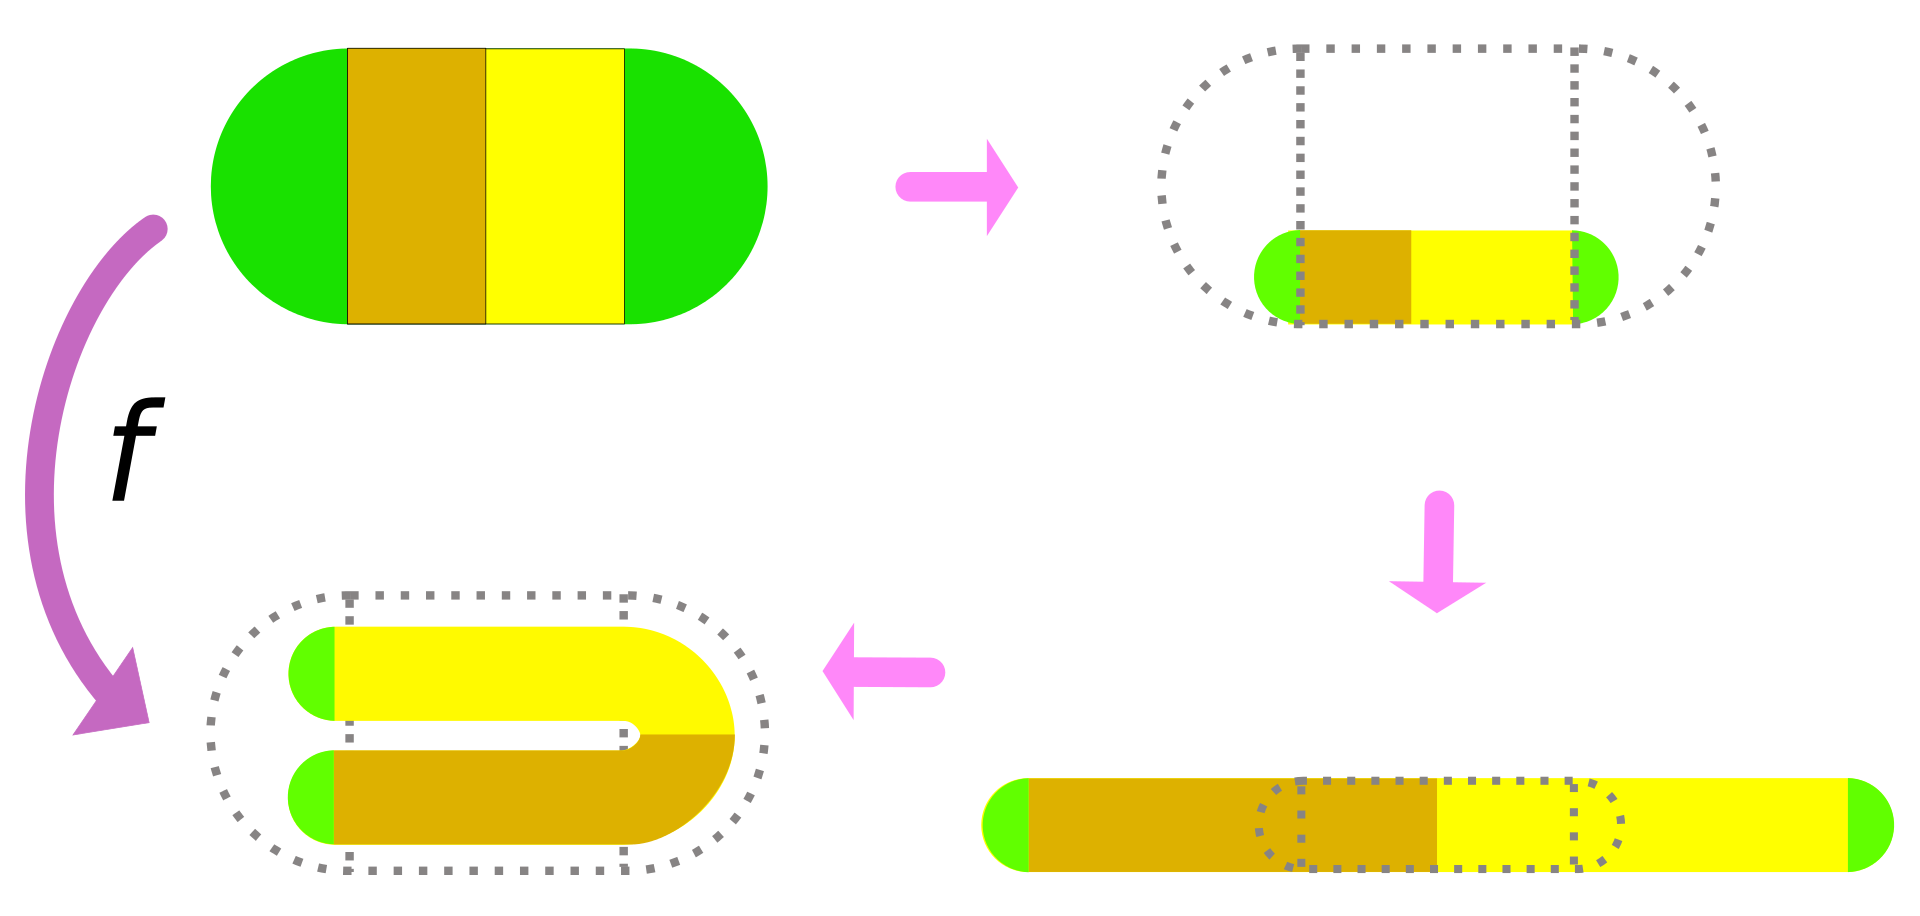
\includegraphics[width=0.4\textwidth]{figures/horseshoe.png}
    \caption{\scriptsize Step della mappa di Horseshoe: meccanismo di Stretching e Folding (wikipedia).}
    \label{fig:figures-horseshoe-png}
\end{figure}
\noindent
Le iterazioni di questa mappa, se sezionate centralmente, portano alla luce un famoso frattale: l'insieme di Cantor.
\begin{figure}[H]
    \centering
    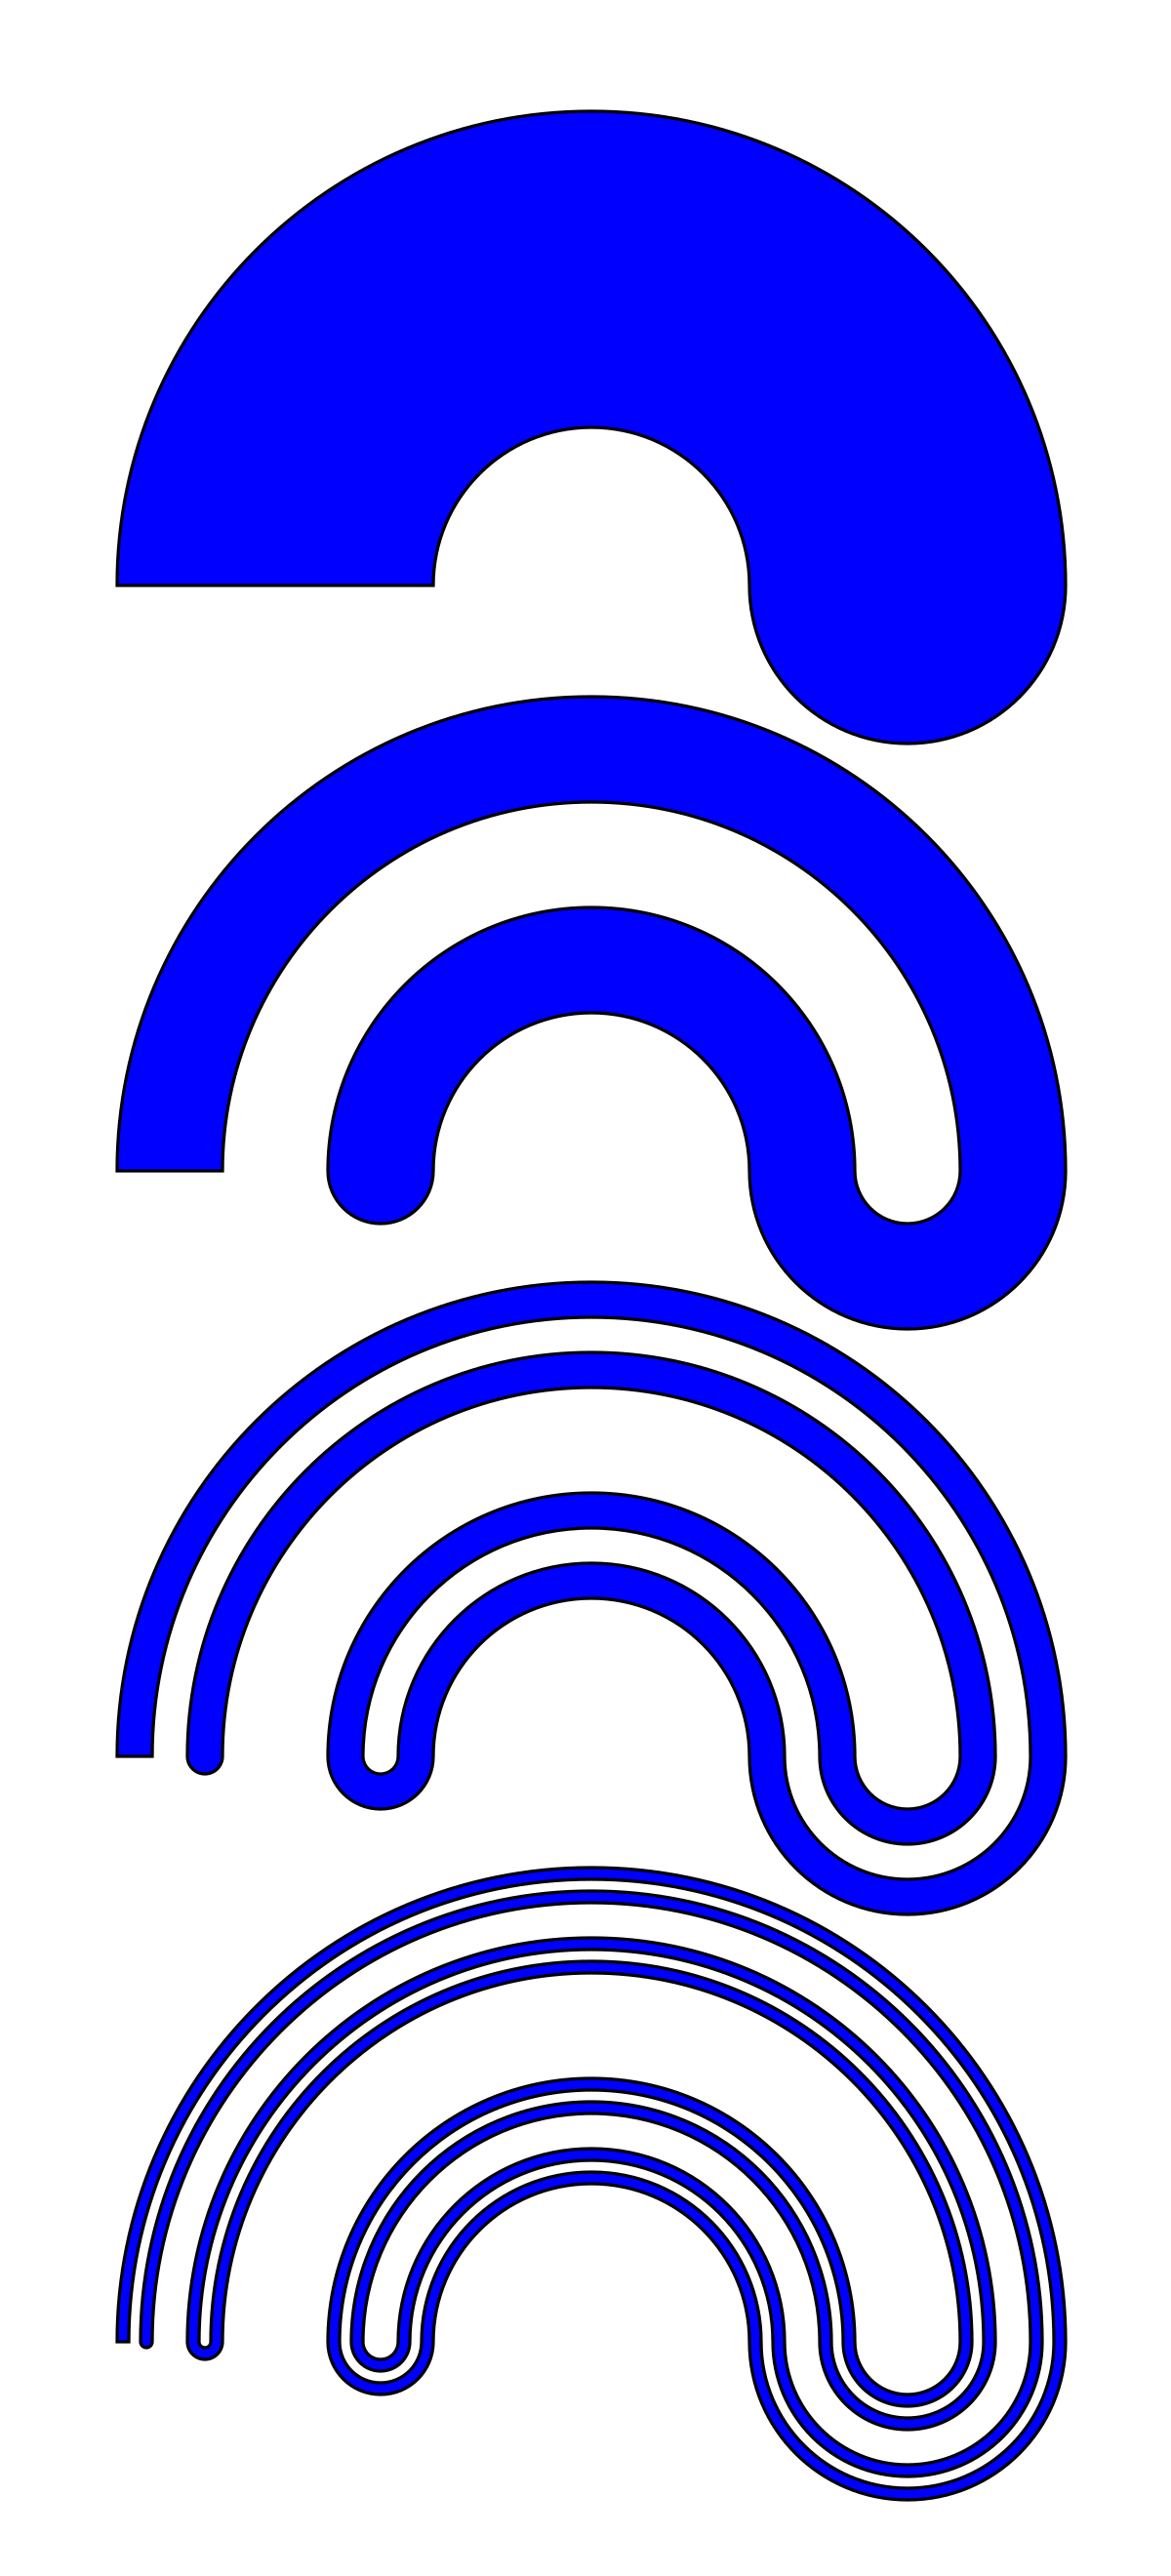
\includegraphics[width=0.2\textwidth]{figures/cantor-horse.png}
    \caption{\scriptsize Iterazioni successive della mappa (viste in un sistema "distorto").\\
    Sezionando la mappa centralmente si ottengono gli step dell'insieme di Cantor.}
    \label{fig:figures-cantor-horse-png}
\end{figure}
\noindent
Il meccanismo di Stretching e Folding porta quindi naturalmente a delle strutture frattali.
\subsubsection{Meccanismo di Period Dubling}%
\label{subsub:Meccanismo di Period Dubling}
Questo meccanismo viene spesso applicato alla mappa logistica come esempio principale, tale mappa è stata ampiamente commentata nella sezione \ref{sub:Mappa logistica}.\\
Abbiamo visto che nella mappa logistica all'aumentare di $\lambda$ le biforcazioni aumentano e di conseguenza aumentano i punti di equilibrio stabile fino all'emergere del caos per un determinato $\overline{\lambda}$ (calcolato da Feigennbaum utilizzando il gruppo di Rinormalizzazione). \\
Ci concentriamo qui sul caso $\lambda  = 1 (> \overline{\lambda})$. Per questo speciale valore di $\lambda$ il sistema diventa uniformemente caotico ed è ergodico.\\ 
Con $\lambda = 1$  la mappa si presenta nella forma:
\[
    x_{n+1}=4(1-2x_n)x_n
.\] 
Effettuando il cambio di variabili:
\[
    x = \frac{1}{2}(1+y)
.\] 
Otteniamo una nuova mappa molto simile a quella di Henon:
\[
    \begin{cases}
        y_{n+1}=1-2y_{n}^2\\
	x_{n+1} = 1 /2(y_n + 1) \qquad -1 \le y_n \le 1
    \end{cases}
\] 
Anche questa è parente del meccanismo di Stretching e Folding in qualche modo\ldots\\
Se cambiamo nuovamente variabili chiamando $y = \sin\theta$  allora la mappa per gli angoli è:
\[
    \theta_{n+1} = \arcsin (\cos (\theta_n)) \implies  \theta_{n+1} = 2\theta_n + \frac{\pi}{2}
.\] 
In cui $\theta$ è mod$\pi$.\\
Questa mappa riempie uniformemente il segmento $\left[0, \pi\right]$.
\clearpage
